\section{Numerical Methods}
\noindent\rule[\linienAbstand]{\linewidth}{\linienDickeDick}
\begin{equation}
  \begin{split}
    h =& t_{k+1} - t_k\\
    t_k =& t_0 + k \cdot h, \;\; k \in mathh{N}
  \end{split}
\end{equation}

\subsection{Explicit Eulers Method}
\noindent\rule[\linienAbstand]{\linewidth}{\linienDicke}
\begin{equation}
  \begin{split}
    \dot{x} &= f(t, x)\\
    x_{k+1} &= x_k + h \cdot f(t_k, x_k)
  \end{split}
\end{equation}

\subsection{Midpoint Method}
\noindent\rule[\linienAbstand]{\linewidth}{\linienDicke}
\begin{equation}
  \begin{split}
    x_{k+\frac{1}{2}} &= x_k + \frac{h}{2} \cdot f(t_k, x_k)\\
    x_{k+1}           &= x_k + h \cdot f(t_{k+\frac{h}{2}}, x_{k+\frac{1}{2}})
  \end{split}
\end{equation}

\subsection{Runge-Kutta Method}
\noindent\rule[\linienAbstand]{\linewidth}{\linienDicke}
\begin{equation}
  \begin{split}
    k_1 &= f(t_k, x_k)\\
    k_2 &= f(t_k + \frac{h}{2}, x_k + \frac{h}{2}k_1)\\
    k_2 &= f(t_k + \frac{h}{2}, x_k + \frac{h}{2}k_2)\\
    k_2 &= f(t_k + h, x_k +h \; k_3)\\
    x_{x+1} &= x_k + \frac{h}{6}(k_1 + 2k_2 + 2k_3 + k_4)
  \end{split}
\end{equation}

\begin{figure}[H]
  \centering
  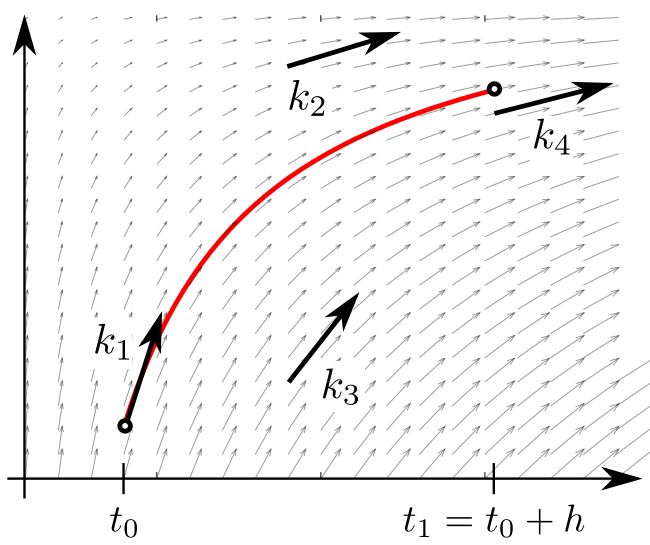
\includegraphics[width=0.5\linewidth]{Pics/runge.png}
\end{figure}
